\section{Entity-Relationship Schema}
Figure 1 shows the entity-relationship schema. Entities are drawn as rectangles, relationships as diamonds, and attributes as circles; filled circles denote the identifiers. Every entity is identified by a surrogate identifier (a UUID generated by the system), since natural keys such as the username or the course code may change over time; those natural keys are nevertheless unique, as stated in the external constraints.

The schema is centred on two entities: \textit{User}, connected to the activities a person performs (roles, enrolments, notifications, quizzes, assignments, resources), and \textit{Course}, which contains the sections, the files and the teaching activities.

\begin{figure}[p]
    \centering
    \makebox[\textwidth][c]{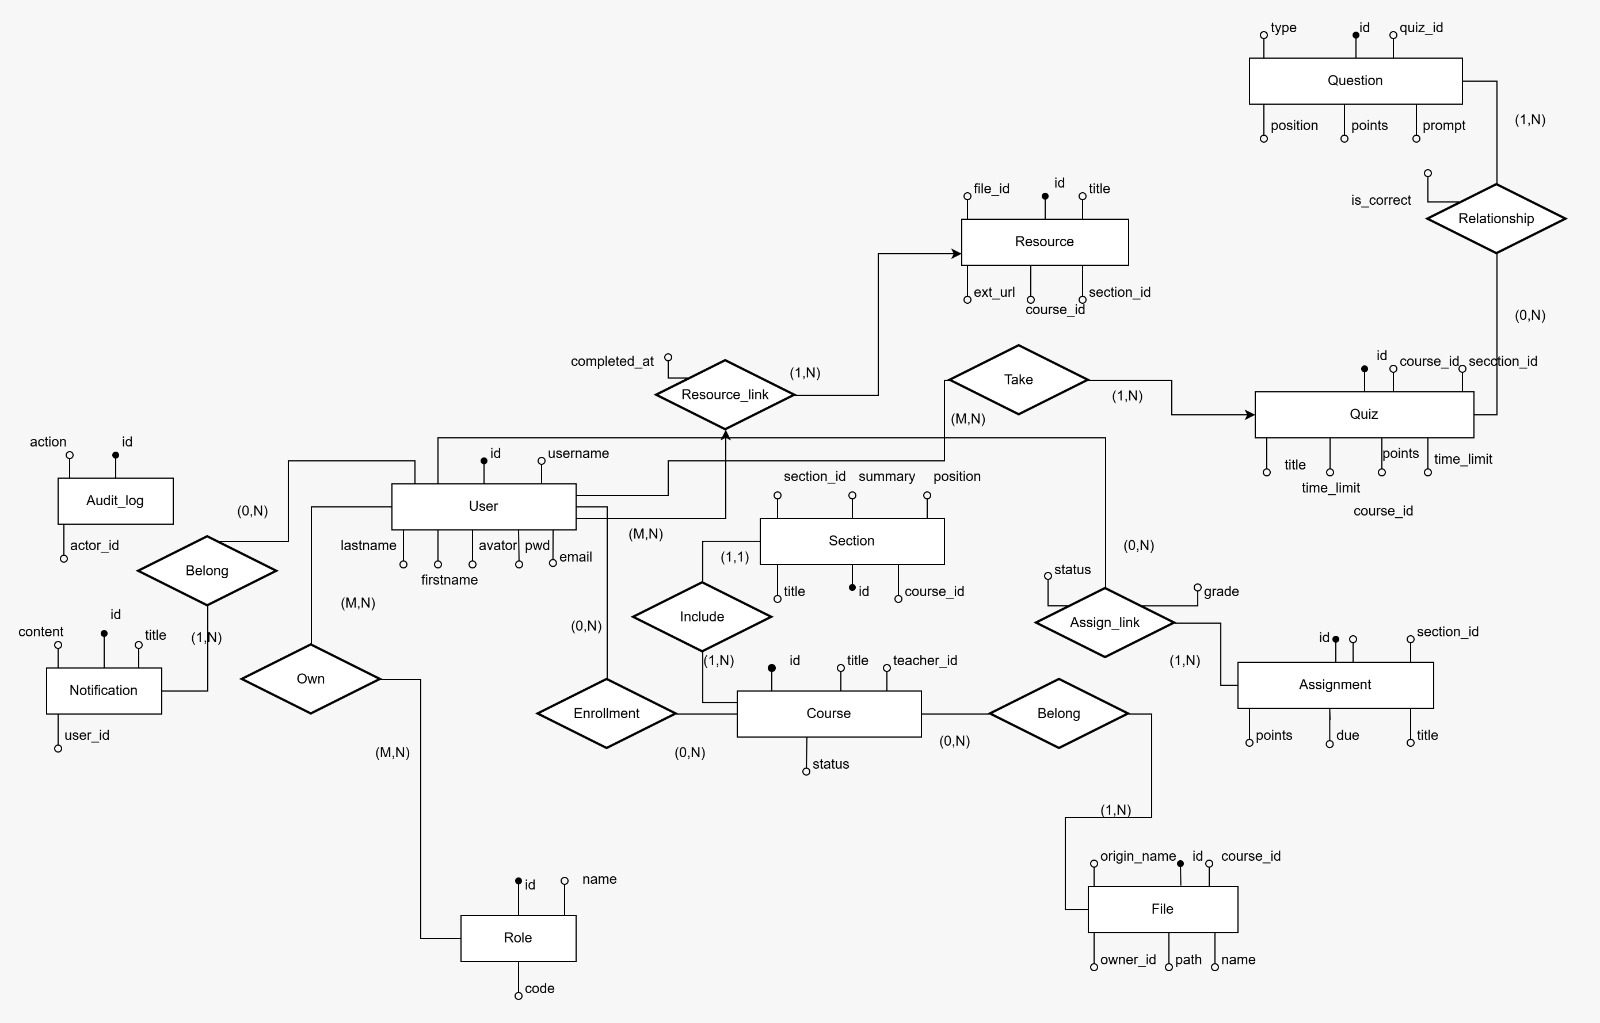
\includegraphics[width=185mm]{figures/er_schema.png}}
    \caption{Entity-Relationship Schema}
    \label{fig:er}
\end{figure}
\clearpage